\documentclass[../../main.tex]{subfiles}
\begin{document}
\onlyinsubfile{
\setcounter{chapter}{0}
}
\notinsubfile{}
\section{Wat zie je?}\label{sec:watzieje}

\marginpar{\hfill\fbox{
\begin{minipage}[t]
{0.9\marginparwidth}naam:\hfill\vspace{1cm}
\end{minipage}
}}
\marginpar{\hfill\fbox{
\begin{minipage}[t]
{0.9\marginparwidth}klas:\hfill\vspace{1cm}
\end{minipage}
}}
\marginpar{\hfill\fbox{
\begin{minipage}[t]
{0.9\marginparwidth}datum:\hfill\vspace{1cm}
\end{minipage}
}}

\begin{center}
\leavevmode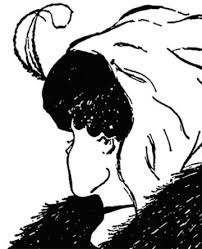
\includegraphics[width=0.5\textwidth]{./img/ovjv.png}
 \captionof{figure}{Oude vrouw jonge vrouw.
\label {fig:wbovjv}}
\end{center}
\nogdoen{niet meer in sync met niet-ingevulde versie}
\paragraph{eerste deel}Zorg dat je een notitieblaadje hebt en een pen in de aanslag. Kijk naar de afbeelding in figuur~\ref{fig:wbovjv}. Je ziet af en toe een jonge vrouw, en af en toe een oude vrouw. 
\iffalse%-k-k-k-k
Sluit het apparaat aan op een USB voeding. Druk op reset om het apparaat startklaar te maken. 
In figuur~\ref{fig:wbovjv} zie je een oude vrouw \'of een jonge vrouw, maar nooit twee tegelijk. Welk beeld je ziet wisselt af. Je hebt dat niet echt onder controle. De oude vrouw en de jonge vrouw kijken naar links. De oude vrouw naar voren, iets omlaag; de jonge vrouw kijkt naar achteren. Het schakelaartje kun je met je linkerhand bedienen. Zodra je het beeld ziet veranderen zet je de schakelaar in de richting waarin de vrouw kijkt: naar beneden als je de oude vrouw ziet, naar boven als je de jonge vrouw ziet.
\fi%-k-k-k-k

Je gaat gedurende \SI{60}{\second} het wisselen waarnemen. Als je docent 
'nu' zegt turf je een 'J' of bij 'O', afhankelijk welk beeld je op dat moment ziet. 

Noteer in de eerste regel in de tabel hieronder het aantal keren dat je 'jonge vrouw' en 'oude vrouw' geturfd hebt  in de tabel.

\begin{tabular}{l|l|l||l|l|l}
                  & jong & oud &                 & jong & oud \\ \hline
jouw waarnemingen &      &     & klas (totaal)   &  64  & 58    \\ \hline
kans              &      &     & kans            &   0,524 & 0,475 \\ \hline
amplitude     &      &     & apmplitude  &   0,724 & 0,689
      
\end{tabular}

\vspace{.5cm}
Iemand verzamelt de gegevens van alle leerlingen in een spreadsheet tabel en telt de totalen op. Je eigen gegevens verwerk je op dit blad, nadat je de rest van paragraaf~\ref{sec:qubits} bestudeerd hebt.


\paragraph{tweede deel} Je bent nu bekend met de braket notatie, en kunnen we met onze persoonlijke resultaten onze eigen toestandsvector $\ket{\Psi}$ tekenen. 
 Daarin stel je de co\"effici\"enten op van de toestand \[\ket{waarneming}=a\ket{O}+b\ket{J}\] uit je eigen meting.

In figuur~\ref{fig:wbkwadrant} vind je een diagram waar je de mate waarin je een oude of een jonge vrouw ziet kunt weergeven.


Bereken de co\"ordinaten van jouw  waargenomen 'toestandsvector' (W) en die van het klassegemiddelde (K) en teken beide in het diagram. 


\vspace{1cm}
%\begin{center}
%\leavevmode
\begin{figure}[ht]
\def\ojfrangle{0}
\def\ojobangle{46.4}%uitgerekend
\def\ojscale{1}
\begin{tikzpicture}%
\begin{scope}[scale=\ojscale, rotate=\ojfrangle]
  \draw[thin,gray!40] (-0.1,-0.1) grid (5,5);
  \draw[-stealth] (-0.1,0)--(5*cos{\ojobangle},0) 
%        node[midway, below, xshift=0]
%        {${\scriptstyle\braket{oude vrouw}{\Psi}}$}
;
  \draw[-stealth] (0,-0.1)-- (0,5*sin{\ojobangle}) 
%        node[midway, left, yshift=0]
%        {${\scriptstyle\braket{jongevrouw}{\Psi}}$}
;
  \node[above] at (0,5) {$\ket{J}$};
  \node[right] at (5,0) {$\ket{O}$};
  \draw[line width=.1pt ,black] ([shift=(0:5)]0,0) arc (0:90:5);
  \draw[thick, red, -stealth](0,0)--(\ojobangle:5)
       node[label={[above, right]$\ket{\Phi}$}] (p){};
  \draw[line width=1pt,dotted] (0,5*sin{\ojobangle}) -- (p);
  \draw[line width=1pt,dotted] (p)--(5*cos{\ojobangle},0);
\end{scope}
\end{tikzpicture}
 \captionof{figure}{Teken hier je eigen toestandvectoren van jouw (W) en het klassengemiddlede (K).%
\label{fig:wbkwadrant}}
\end{figure}
%\end{center}


\nogdoen{Met welke bewerking kom je van kansamplitude naar kans?
Vergelijk waarneming proef van young en licht}

\notepadlines[5]
\vspace{0.25in}
 
\end{document}
